\chapter{Introduction to Object-Oriented Programming (OOP) Concepts}

\section{Introduction: Real-Life Hook}

Ayesha is a high school student who keeps information about her classmates:
names, roll numbers, and marks.

At first, she writes separate variables:
\begin{itemize}
    \item \texttt{name1, roll1, marks1}
    \item \texttt{name2, roll2, marks2}
\end{itemize}

Very soon, her code becomes confusing and messy.

She asks:
``Is there a better way to organize related data and actions together?''

The answer is \textbf{Object-Oriented Programming (OOP)}.

\section{Concept: What Is Object-Oriented Programming?}

\begin{definition}{Object-Oriented Programming}
Object-Oriented Programming (OOP) is a programming approach where \textbf{data and functions are grouped together into objects}.
\end{definition}

OOP helps us:
\begin{itemize}
    \item Organize code clearly
    \item Model real-world things
    \item Reuse and manage large programs easily
\end{itemize}

\section{Real-Life Example of OOP}

Think about a \textbf{student}.

A student has:
\begin{itemize}
    \item Data: name, roll number, marks
    \item Actions: \texttt{study()}, \texttt{take\_exam()}, \texttt{show\_result()}
\end{itemize}

In OOP:
\begin{itemize}
    \item Data $\rightarrow$ \textbf{attributes}
    \item Actions $\rightarrow$ \textbf{methods}
\end{itemize}

\section{Basic OOP Terms}

\subsection{Class}

\begin{definition}{Class}
A class is a \textbf{blueprint or template} used to create objects.
\end{definition}

Example:
\begin{verbatim}
class Student:
    pass
\end{verbatim}

\subsection{Object}

\begin{definition}{Object}
An object is a \textbf{real instance of a class}.
\end{definition}

Example:
\begin{verbatim}
s1 = Student()
s2 = Student()
\end{verbatim}

\section{Attributes and Methods}

\subsection{Attributes (Variables inside a class)}

\begin{verbatim}
class Student:
    def __init__(self, name, roll):
        self.name = name
        self.roll = roll
\end{verbatim}

\subsection{Methods (Functions inside a class)}

\begin{verbatim}
class Student:
    def __init__(self, name, roll):
        self.name = name
        self.roll = roll

    def display(self):
        print("Name:", self.name)
        print("Roll:", self.roll)
\end{verbatim}

\section{Creating and Using Objects}

\begin{verbatim}
s1 = Student("Ayesha", 5)
s2 = Student("Rafi", 8)

s1.display()
s2.display()
\end{verbatim}

Each object has its \textbf{own data}, even though they use the same class.

\section{Why Use OOP?}

\begin{itemize}
    \item Groups related data and actions together
    \item Makes code easier to understand
    \item Helps manage large projects
    \item Matches real-life thinking
\end{itemize}

\section{Mini-Project: Student Information System}

\textbf{Goal:} Store and display student information using OOP.

\begin{verbatim}
class Student:
    def __init__(self, name, marks):
        self.name = name
        self.marks = marks

    def result(self):
        if self.marks >= 40:
            print(self.name, "has passed")
        else:
            print(self.name, "has failed")

s1 = Student("Ayesha", 75)
s2 = Student("Rafi", 32)

s1.result()
s2.result()
\end{verbatim}

Students learn:
\begin{itemize}
    \item Class creation
    \item Object creation
    \item Using methods
\end{itemize}

\section{Diagram: Class and Object Relationship}

\begin{center}
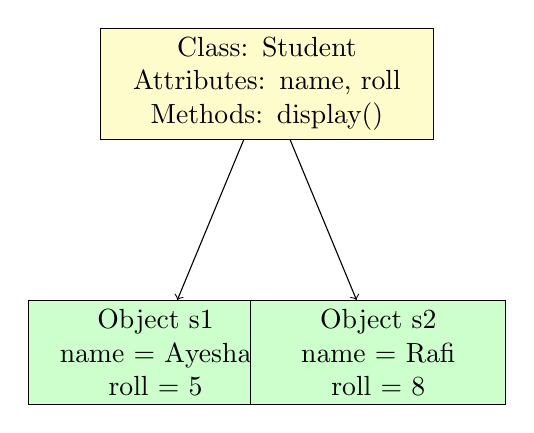
\begin{tikzpicture}[node distance=2cm]
\node (class) [draw, rectangle, fill=yellow!20, text width=4cm, align=center] {Class: Student\\
Attributes: name, roll\\
Methods: display()};
\node (obj1) [draw, rectangle, fill=green!20, below left of=class, yshift=-2cm, text width=3cm, align=center] {Object s1\\
name = Ayesha\\
roll = 5};
\node (obj2) [draw, rectangle, fill=green!20, below right of=class, yshift=-2cm, text width=3cm, align=center] {Object s2\\
name = Rafi\\
roll = 8};

\draw[->] (class) -- (obj1);
\draw[->] (class) -- (obj2);
\end{tikzpicture}
\end{center}

\section{Key Concepts}

\begin{itemize}
    \item OOP models real-world entities
    \item Class is a blueprint
    \item Object is an instance of a class
    \item Attributes store data
    \item Methods define behavior
\end{itemize}

\section{End-of-Chapter Exercises}

\subsection{Very Short Questions}

\begin{enumerate}
    \item What is OOP?
    \item What is a class?
    \item What is an object?
\end{enumerate}

\subsection{Short Answer Questions}

\begin{enumerate}
    \item Explain the difference between a class and an object.
    \item Define attributes and methods with examples.
    \item Why is OOP useful in large programs?
\end{enumerate}

\subsection{Activity-Based Exercises}

\begin{enumerate}
    \item Create a \texttt{Book} class with attributes title and author.
    \item Create a \texttt{MobilePhone} class with methods \texttt{call()} and \texttt{message()}.
    \item Modify the Student class to include grade calculation.
\end{enumerate}

\section{Teacher Notes}

\marginnote{
\textbf{Learning Objectives}
\begin{itemize}
    \item Understand basic OOP concepts
    \item Create classes and objects
    \item Relate programming to real-life examples
\end{itemize}

\textbf{Teaching Tips}
\begin{itemize}
    \item Use classroom objects (chair, student, board) as examples
    \item Draw class-object diagrams on the board
    \item Let students design their own classes
\end{itemize}

\textbf{Assessment}
\begin{itemize}
    \item Correct class and object creation
    \item Proper use of attributes and methods
\end{itemize}
}